\documentclass[tikz,border=2pt]{standalone}
\usepackage{amsmath,graphicx}
\usepackage{xcolor}

\definecolor{hexfg}{HTML}{D2DC46}
\definecolor{hexbg}{HTML}{00008C}
%\definecolor{hexbg}{HTML}{001450}
\definecolor{titlecol}{HTML}{FFFFFF}


\begin{document}
\begin{tikzpicture}
  % background
  \fill[hexbg]
    (90:3) -- (150:3) -- (210:3) -- (270:3) -- (330:3) -- (30:3) -- cycle;
  % border
  \draw[hexfg, line width=4pt, line join=round]
    (90:3) -- (150:3) -- (210:3) -- (270:3) -- (330:3) -- (30:3) -- cycle;

  \begin{scope}[text=hexfg]
  
   
   \node[text=titlecol] at (-0.1, 1.6) {\sffamily\bfseries\LARGE simecol};
    \node at (-0.1, 1.0) {\scalebox{0.7}{\sffamily\bfseries simulation of ecological models}};
    
    \node at (-0.3,-0.1) {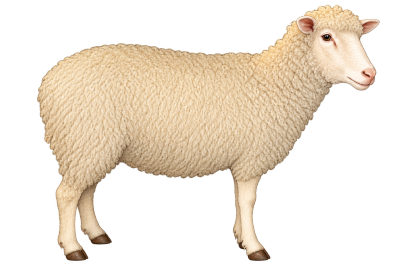
\includegraphics[width=2cm]{sheep-small.png}};
    \node at ( 0.3,-0.9) {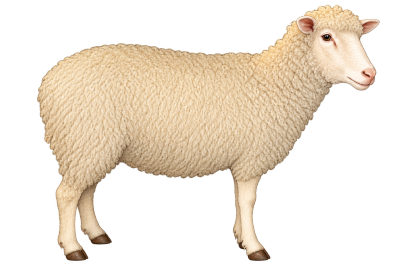
\includegraphics[width=2cm]{sheep-small.png}};
    
    
    \node at (-0.1,-1.8) {\scalebox{0.7}{\sffamily\bfseries ODE -- CA -- IBM/ABM}};
   
    
    %\node at (0,1.8) {$\left[\begin{matrix}
    %    \text{\sffamily\scriptsize ODE},\text{\sffamily\scriptsize DDE}\\
    %    \text{\sffamily\scriptsize PDE},\text{\sffamily\scriptsize DAE}
    %  \end{matrix}\right]$};

  \end{scope}
\end{tikzpicture}
\end{document}

% pdftocairo -svg desolve-logo.pdf desolve-logo.svg
